\subsection*{Модель взаимодействия центра и переферии}
\addcontentsline{toc}{subsection}{Модель взаимодействия центра и переферии}

\textbf{Задание:}\\
Провести численный анализ модели взаимодействия центра и переферии в среде AnyLogic.\\

\textbf{Решение:}\\
$N_c$ -- численность населения центра\\
$N_p$ -- численность населения периферии\\
$T_c$ -- техническое развитие центра\\
$T_p$ -- техническое развитие переферии\\
$E_c$ -- уровень грамотности центра\\
$E_p$ -- уровень грамотности переферии\\
$Y_c$ -- величина ВВП центра\\
$Y_p$ -- величина ВВП переферии\\
$e_c$ -- отношение числа работающего населения ко всему населению в центре\\
$e_p$ -- отношение числа работающего населения ко всему населению в переферии\\
$C$ -- функция связи

\begin{align*}
& \dfrac{dN_c}{dt} = a_c T_c N_c (1 - E_c) + a' N_p C_N\\
& \dfrac{dT_c}{dt} = b_c T_c E_c\\
& \dfrac{dE_c}{dt} = c_c T_c E_c (1 - E_c)\\
& Y_c = e_c T_c N_c\\
& \dfrac{dN_p}{dt} = a_p T_p N_p (1 - E_p) + a' N_p C_N\\
& \dfrac{dT_p}{dt} = b_p T_p E_p + b' T_c C_T\\
& \dfrac{dE_p}{dt} = c_p T_p E_p (1 - E_p) + c' E_c C_E\\
& Y_p = e_p T_p N_p\\
\end{align*}

\newpage

В соответствии с формулами, данная модель была реализована в среде моделирования AnyLogic. (Рисунок \ref{fig:center1})
\begin{figure}[h]
	\centering 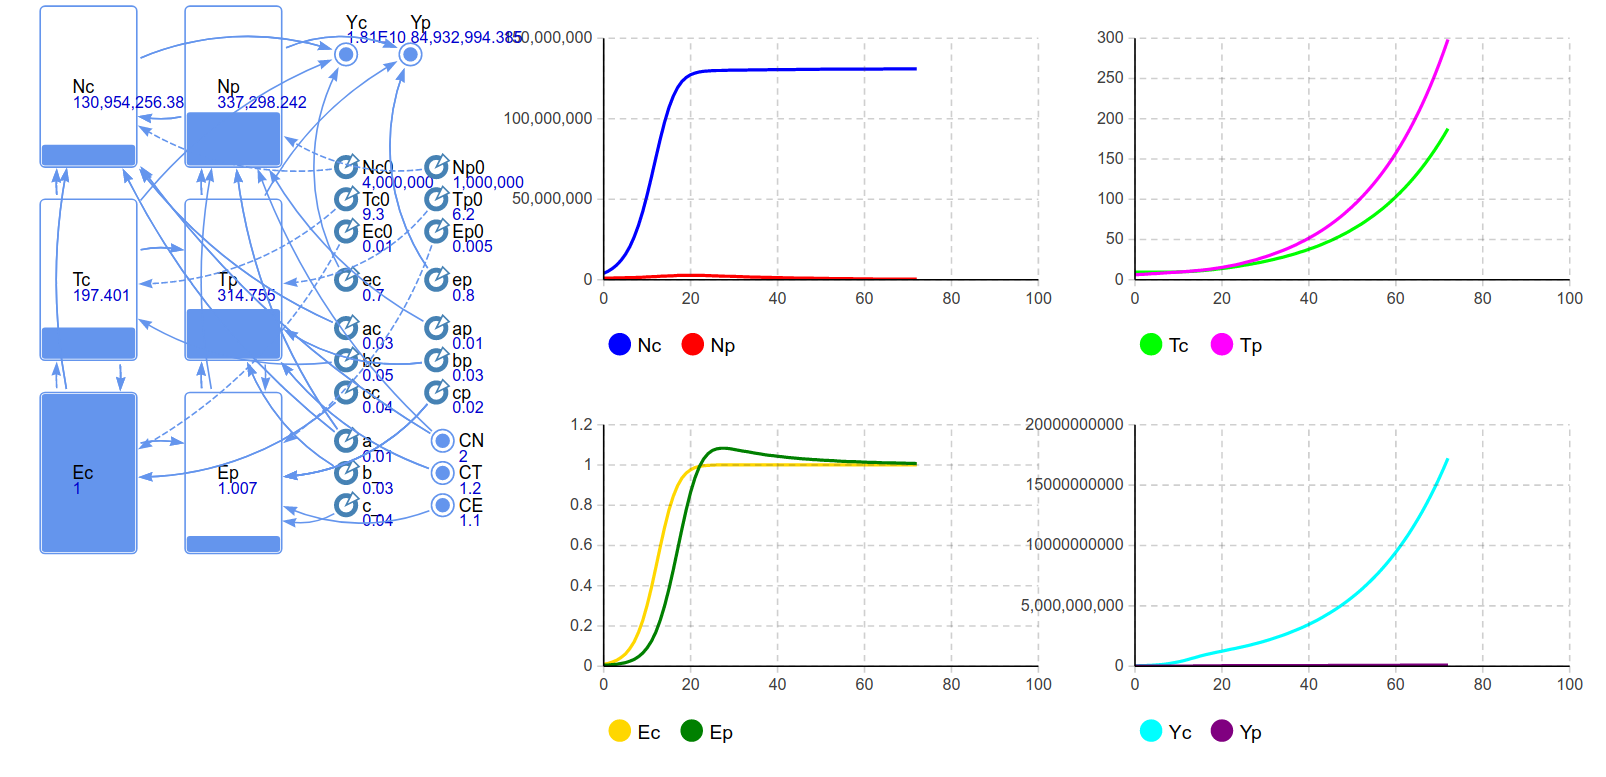
\includegraphics[scale=0.23]{center1}
	\caption{Результаты построения модели взаимодействия центра и переферии в AnyLogic}
	\label{fig:center1}
\end{figure}

Модель подчиняется нескольким следующим соображениям:
\begin{enumerate}[topsep=0pt,itemsep=-1ex,partopsep=1ex,parsep=1ex]
	\item Технологическое развитие центра растет в значительной мере быстрее чем технологическое развитие периферии, обмениваясь с периферией технологиями.
	\item Культурное развитие растет примерно одинаковыми темпами, однако темпы роста культурного развития центра превышают темпы культурного развития периферии.
	\item Население периферии растет быстрыми темпами, а население центра растет очень медленно, но засечёт миграции темпы роста увеличиваются, однако все равно остаются гораздо ниже темпов роста населения периферии.
	\item Несмотря на то, что доля работоспособного населения на периферии больше, чем в центре, значение ВВП периферии ниже, чем у центра.
\end{enumerate}

\newpage

Теперь можно поменять значения функции связи и посмотреть что получится в результате данного изменения. (Рисунок \ref{fig:center2})
\begin{figure}[h]
	\centering 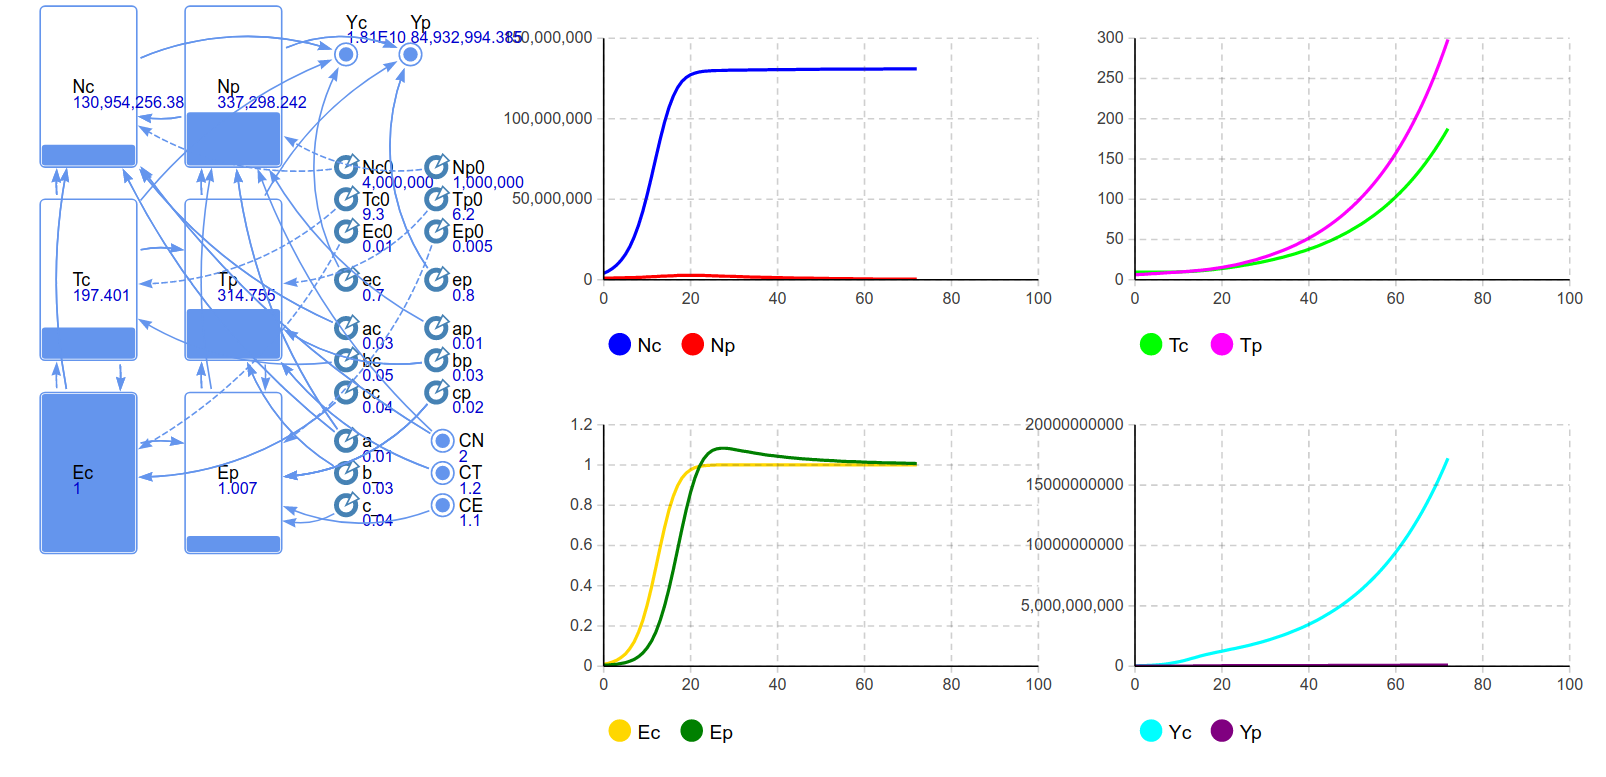
\includegraphics[scale=0.23]{center1}
	\caption{Результаты построения модели взаимодействия центра и переферии в AnyLogic}
	\label{fig:center2}
\end{figure}

Можно видеть, что после увеличения значения функции технического развития увеличиваются темпы роста технического развития переферии.\\

Схожая ситуация наблюдается при изменении значения функции связи культурного развития.

Таким образом, была реализована модель взаимодействия центра и переферии при различных параметрах.